\documentclass[paper=a4wide, fontsize=10pt]{scrartcl}	 % A4 paper and 11pt font size
\usepackage[portuguese]{babel}
\usepackage{booktabs}
\usepackage{mathtools}
\usepackage{amssymb}
\usepackage[svgnames]{xcolor} % Using colors
\usepackage{background} % To include background images
\usepackage{amsmath}
\usepackage{fancyhdr} % Needed to define custom headers/footers
\usepackage[a4paper, left=20mm, right=20mm, top=20mm, bottom=2cm, footskip=1.2cm]{geometry}  % Changing size of document
%\usepackage[square, numbers, comma, sort&compress]{natbib} % Use the natbib reference package - read up on this to edit the reference style; if you want text (e.g. Smith et al., 2012) for the in-text references (instead of numbers), remove 'numbers'
\newcommand*\dif{\mathop{}\!\mathrm{d}}
\newcommand{\naturais}{\mathbb{N}}
\newcommand{\reais}{\mathbb{R}}
\newcommand{\Esp}[1]{\mathbb{E}[#1]}
\newcommand{\EspMonstro}[1]{\mathbb{E}\Bigg[#1\Bigg]}
\newcommand{\Vari}[1]{\mathbb{V}\text{ar}[#1]}
\newcommand{\VariMonstro}[1]{\mathbb{V}\text{ar}\Bigg[#1\Bigg]}
\newcommand{\Estim}[1]{\hat{#1}}
\newcommand{\Norm}[2]{\mathcal{N}(#1#2)}
\newcommand{\Vies}[1]{\mathbb{B}[#1]}
\newcommand{\Prob}[1]{\mathbb{P}\left(#1\right)}
\newcommand{\ProbMonstro}[1]{\mathbb{P}\Bigg(#1\Bigg)}
\newcommand{\Cova}[1]{\mathbb{C}\text{ov}[#1]}
\newcommand{\CovaMonstro}[1]{\mathbb{C}\text{ov}\Bigg[#1\Bigg]}
\usepackage[alf]{abntex2cite}  % Citações padrão ABNT
\usepackage{braket}
\usepackage{float}

%%%%%% Setting up the style

\setlength\parindent{0pt} % Gets rid of all indentation
\backgroundsetup{contents={\includegraphics[width=\textwidth]{logo.jpg}},scale=0,placement=top,opacity=1,position={7.2cm,2cm}} %  OIST Logo
\pagestyle{fancy} % Enables the custom headers/footers

\lhead{} \rhead{} % Headers - all  empty

\definecolor{emerald}{RGB}{0,155,119}
\definecolor{RedHeat}{RGB}{152,0,46}
\definecolor{EgyptianBlue}{RGB}{2,45,180}


\title{\vspace{-1cm}  \color{emerald} Relatório de Pesquisa - MAP2212 - EP1}
\subtitle{Cálculo do \(\pi\) através do método de Monte Carlo % Title of the rotation project
\vspace{0.3cm} }
\date{} % No date

\lfoot{\color{EgyptianBlue} Guilherme Dias Vianna \& Michel Csillag Finger }  % Write your name here
\rfoot{\color{RedHeat} IME-USP}


\renewcommand{\headrulewidth}{0.0pt} % No header rule
\renewcommand{\footrulewidth}{0.4pt} % Thin footer rule

%%%%%% Starting the document

\begin{document}

\maketitle % Print the title
\thispagestyle{fancy} % Enabling the custom headers/footers for the first page


% In the following lines, add the relevant information
\vspace{-1.5cm} \textbf{Nome:} Guilherme Dias Vianna (NUSP: 9301429)

\textbf{Nome:} Michel Csillag Finger (NUSP: 5490532)

\textbf{Data de Entrega:} 16/03/2024

\textbf{Professor:} Julio Michael Stern

\textbf{Unidade:} IME - USP



\section{Objetivo}
    O objetivo deste exercício é estimar a constante \(\pi\) com uma precisão dada (sem conhecimento prévio do valor) utilizando um algoritmo de Monte Carlo.

    O algoritmo em questão utilizado será o de gerar \(n\) pontos aleatórios pertencentes ao quadrado de lado 2:

    \[
    \{(x_i,y_i)\}_{i=1}^n \in [-1,1]\times[-1,1]
    \]

    E observar quantos se encontrarão dentro do círculo unitário:

    \[
    \mathcal{C}_1 = \{(x,y)\in\mathbb{R}^2 : x^2+y^2\leqslant1\}
    \]

    Pela \textbf{Lei dos Grandes Números}\cite{Gut2005-GUTPAG}, é esperado que a razão do número de pontos dentro do círculo em relação ao total de pontos se aproxime da razão entre as áreas:

    \[\frac{\text{Número de pontos em \(\mathcal{C}_1\)}}{\text{Número total de pontos gerados}} \xrightarrow{n\rightarrow +\infty} \frac{\pi}{4}\]

   Resta agora saber qual será um bom \(n\) para que nossa estimativa seja, mesmo sem saber \textit{a priori} o valor de \(\pi\), para que a precisão de nossa estimativa seja menor que um dado \(\epsilon\).

    \begin{figure}[h!]
    \centering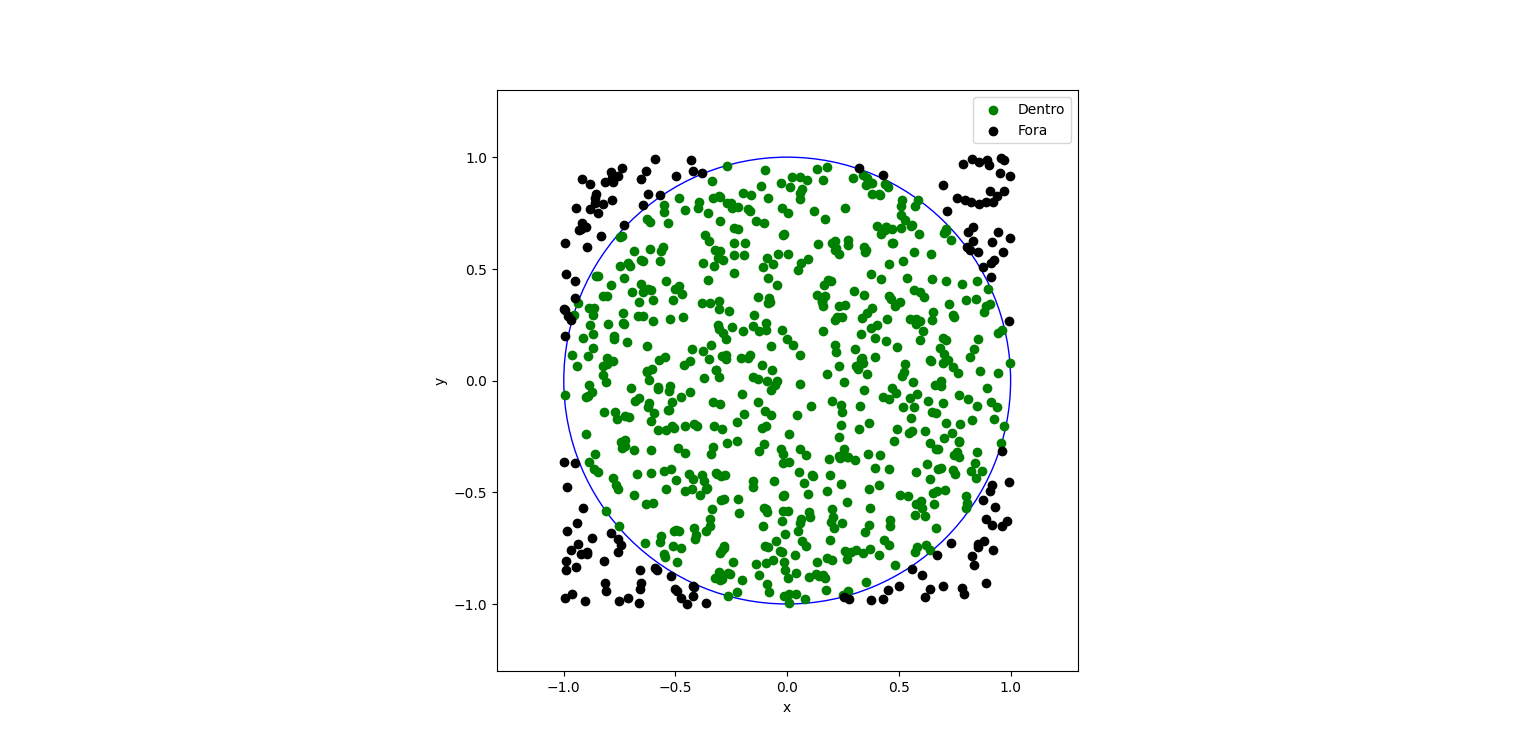
\includegraphics[width=1.1\linewidth]{Figure_1.png}
    \caption{Ideia do experimento.}
\end{figure}
   
\section{Preparativos}

\subsection{Uma primeira aproximação}

    Primeiramente é importante ter alguma noção de uma cota inferior e superior para \(\pi\).

    \begin{itemize}
        \item 
        Como a área do quadrado é \(4\), a área do círculo é \(\pi\) e o círculo está contido no quadrado, temos que:

        \[
        \pi < 4
        \]
        
        \item
        Como dentro de uma circunferência temos\footnote{Como o foco deste trabalho não é sobre geometria plana, apenas indicamos a demonstração desse fato em \cite{dolce2013fundamentos}} um dodecágono regular, composto de \(12\) triângulos regulares de área \(1/4\), temos então que:

        \[
        \pi > 12 \cdot \frac{1}{4} = 3
        \]

        Combinado ambas temos que:

        \[
        3<\pi<4
        \]
        
    \end{itemize}

Isso já nos dá uma primeira aproximação e um intervalo para se manter em mente ao lançar mão de alguma outra técnica ou método de estimação.

\subsection{Uma descrição estatística da simulação}

O algoritmo de Monte Carlo utilizado consistirá de:

\begin{enumerate}
    \item Gerar \(n\) valores \(X_i \sim \mathcal{U}(-1,1)\) e \(n\) valores \(Y_i \sim \mathcal{U}(-1,1)\) independentes
    \item Calculamos a razão entre o número de pontos \(P_i = (X_i,Y_i) \in \mathcal{C}_1\), sobre o número total:

    \[
    \mathcal{R} = \frac{\text{Número de pontos em \(\mathcal{C}_1\)}}{n} 
    \]

\end{enumerate}

Veja que, com isso, o numerador de \(\mathcal{R}\) é dado pela variável aleatória \(S_n\sim \text{Bin}(n,\frac{\pi}{4})\), já que para cada ponto \(P_i\), a probabilidade de estar no interior do círculo é dada por uma variável \(p_i \sim \text{Ber}(\frac{\pi}{4})\).

Veja também que o valor esperado de \(S_n\) é:

\[
\Esp{S_n} = n\frac{\pi}{4}
\]

E com isso:

\[
\Esp{\mathcal{R}} =\frac{1}{n}\Esp{S_n} = \frac{\pi}{4}
\]

\subsection{Estimativa do \(n\) necessário}

Uma estimativa possível de \(n\) para obter a precisão desejada pode ser obtida pela \textbf{Desigualdade de Chebyshev} \cite{Roussas}:

\[
\Prob{\left|X-\Esp{X}\right|>\epsilon}\leqslant \frac{\Vari{X}}{\epsilon^2}
\]

Tomando \(X\) como \(4\mathcal{R}\), ficamos com:

\[
\ProbMonstro{4\left|\frac{S_n-\Esp{S_n}}{n}\right|>\epsilon} \leqslant \frac{\Vari{4\frac{S_n}{n}}}{\epsilon^2}
\]

Desejamos que nossa estimativa de \(4\mathcal{R}\) (representada aqui por \(r\)) seja tal que \(\left|\frac{r-\pi}{\pi}\right|<0,05\%\), como a quantidade dentro do módulo será proporcional a \(\left|r-\pi\right|\) nas simulações, escolhemos então \( \epsilon = 0,05 \pi \% \), substituindo os valores esperados e variâncias e fazendo algumas manipulações:

\[
\ProbMonstro{\left|\frac{4\frac{S_n}{n}-\pi}{\pi}\right|>0,05\%}  \leqslant \frac{16}{n^2\epsilon^2}\Vari{S_n} = \frac{4\pi(1-\frac{\pi}{4})}{n(0,005\pi)^2} = \frac{16000000}{n}\frac{1-\frac{\pi}{4}}{\pi}
\]

Analisemos a seguinte função \(f:\mathbb{R}^*_{+}\rightarrow\mathbb{R}\), dada por:

\[
f(x) = \frac{1-\frac{x}{4}}{x}
\]

Veja que:

\[
\frac{\dif{f}}{\dif{x}} = -\frac{1}{x^2} < 0
\]

Daonde tiramos que \(f\) é estritamente descrescente. Como sabemos que \(\pi > 3\), então temos que \(f(\pi)<f(3)\) 

Com isso podemos escrever então que:
\[
\frac{16000000}{n}\frac{1-\frac{\pi}{4}}{\pi} < \frac{16000000}{n}\frac{1-\frac{3}{4}}{3} = \frac{4000000}{3n}
\]

Com isso obtivemos uma cota superior para a probabilidade da nossa estimativa:

\[
\ProbMonstro{\left|\frac{4\frac{S_n}{n}-\pi}{\pi}\right|>0,05\%}  \leqslant \frac{4000000}{3n}
\]

Agora precisamos arbitrar o \(n\) necessário para que a probabilidade seja baixa (já que gostaríamos que a probabilidade de nossa estimativa ter um erro relativo maior que \(0,05\%\) fosse baixa).

\textbf{Escolhendo} que a probabilidade em questão seja \(5\%\):

\[
0,05 \leqslant \frac{4000000}{3n} \Rightarrow n \geqslant  26666666, 67
\]

Veja que com isso, podemos então concluir que \(n^* = 26666667\) é um tamanho de amostra suficiente para a precisão requisitada. Porém, como serão gerados pontos com duas coordenadas aleatórias, na realidade serão necessários \(2n^* = 53333334\) números sorteados.

\section{Implementação da simulação via \texttt{Python}}

\begin{itemize}

\item {Geração de Pontos Aleatórios:}

Utiliza-se a função \texttt{np.random.uniform(-1, 1, (n, 2))} para gerar \texttt{n} pontos aleatórios. Cada ponto tem coordenadas \texttt{(x, y)}, com \texttt{x} e \texttt{y} distribuídos uniformemente entre -1 e 1, assegurando que os pontos estejam dentro do quadrado de lado 2 centrado na origem.

\item {Determinação de Pontos Dentro da Circunferência:}

Para cada ponto, calcula-se \texttt{x$^2$ + y$^2$} para determinar se o ponto está dentro da circunferência de raio 1. Se \texttt{x$^2$ + y$^2$ $\leq$ 1}, o ponto está dentro da circunferência.

\item {Cálculo da Proporção e Estimativa de $\pi$:}

A proporção de pontos dentro da circunferência (\texttt{proporcao\_dentro}) é calculada dividindo-se o número de pontos dentro pelo total de pontos \texttt{n}. Esta proporção é usada para estimar $\pi$, multiplicando-a por 4 (\texttt{pi\_estimado}).

\item {Avaliação da Precisão da Estimativa:}

A precisão da estimativa de $\pi$ é avaliada calculando-se a diferença percentual entre \texttt{pi\_estimado} e o valor real de $\pi$, usando \texttt{100*np.abs(pi\_estimado - np.pi)/np.pi}, resultando em \texttt{diferenca\_para\_pi}.

\item {Condição de Aceitação:}

O programa verifica se a diferença percentual (\texttt{diferenca\_para\_pi}) excede 0,05\%. Se exceder, indica que a precisão da estimativa não está dentro do critério estabelecido. Caso contrário, considera-se que a estimativa possui uma precisão aceitável.

\item {Execução Repetida:}

O programa executa \texttt{m} vezes a função \texttt{pontos\_dentro\_circunferencia\_e\_figura(n)}, onde \texttt{m} é definido como 10000. Para cada execução, \texttt{n} é fixado em 26666667, o valor obtido pela desigualdade de Chebyshev para alcançar a precisão desejada na estimativa de $\pi$.

\end{itemize}

\section{Resultados e conclusão}

Dentre as 10000 execuções do programa, todas ficaram dentro da margem de tolerância permitida. As possíveis razões para isso são:

\begin{itemize}
    \item Provavelmente se deve a ter uma majoração maior do
que a necessária. 
    \item  A quantidade de pontos é muito alta e como são números
pseudo-aleatórios, o efeito de aleatoriedade simulada é perdido.
\end{itemize}

\bibliography{Bibliografia}



\end{document}
